\section{Joint Planning with Acquired Structural Evidence}
\label{main-method}

\subsection{Measured state and conditional completion}
The mapping backend integrates only acquired RGB-D and scan measurements. Measured occupancy supplies traversability and unknown-space masks; an Open3D CPU TSDF supplies the reconstructed surfaces~\cite{ref4,ref11}. Observed instance tracks associate measured surface patches with objects. Template completion is restricted to these positive tracks, while unassigned geometry still contributes to mapping, collision checking and the common coverage/quality terms. This prevents a small unassigned fragment from independently receiving a whole furniture template. Both G and S receive the same ideal visible instance associations in the virtual tests.

Each modeled object has closed-box and open-shelf alternatives. Their common coordinate frame, width, vertical parts and measured support are estimated from acquired points. Qualified outer faces constrain orientation; measured horizontal faces constrain available layers. These estimates remain imperfect. We represent uncertainty only in local depth and the allocation of unseen extent; orientation, width, layer count and pose are not integrated out. Model mismatch is therefore retained rather than absorbed into a claim of a complete shape posterior.

For object $o$, geometric particle $k=(d,a)$ has depth $d$ and an allocation $a$ of unseen extent around the measured interval. The public depth density is uniform on $[0.2,1.4]$\,m, conditioned on the acquired span. Nodes at 0.1\,m spacing, together with an inserted measured-span boundary, receive clipped Voronoi integration masses. A qualified measured end fixes that coordinate. Without an end anchor, $a\in\{0,0.5,1\}$ has prior masses $\{0.25,0.5,0.25\}$ and places the lower endpoint at measured minimum minus $a(d-\text{span})$. Opposite observed ends fix depth directly. Out-of-support spans and missing/multiple tracks remain explicit failures in independent probability evaluation; its public-prior fallback is an evaluator convention, not hidden ground-truth object selection.

\subsection{Observation loss and structural mixture}
Every alternative is evaluated using the same acquired points and valid depth rays. The loss $E_{ohk}$ adds mean point-to-template squared distance and mean strict-free first-hit depth discrepancy, each clipped at 0.15\,m before squaring. The common ray set encloses all alternatives. A template hit behind a nearer observed hit is occluded; it is not free-space evidence. Invalid depth adds no evidence, and measured surface support vetoes conflicting free-space classification across views. Rebuilding from the acquired state avoids multiplying a previous posterior by the same observations again.

The loss-based distribution~\cite{bissiri2016} uses one externally selected scale $\sigma$:
\begin{equation}
Z_{oh}=\sum_k q_{o0}(k)e^{-E_{ohk}/(2\sigma^2)},\qquad
q_o(k\mid h,\mathcal D_t)=\frac{q_{o0}(k)e^{-E_{ohk}/(2\sigma^2)}}{Z_{oh}}.
\end{equation}
The depth scale is fixed at $0.01$\,m by a separate training CRPS comparison. This generalized loss is not an exact RGB-D sensor likelihood, and its scale does not by itself calibrate structural confidence. We therefore evaluate a declared modular structural-temperature revision:
\begin{equation}
\pi_{o,T}^m(h)=
\frac{\pi_{o,0}^m(h)\exp(\log Z_{oh}/T)}
{\sum_{h'}\pi_{o,0}^m(h')\exp(\log Z_{oh'}/T)},\qquad
w_{ohk}^m=\pi_{o,T}^m(h)q_o(k\mid h,\mathcal D_t).
\label{eq:modular-update}
\end{equation}
G uses $\pi_{o,0}^G=(0.5,0.5)$; S uses the same finite acquired-label vote rule as the preceding implementation. Temperature scaling~\cite{pmlr-v70-guo17a} is applied to structural evidence before category log-odds are added. Any positive $T$ preserves G's class preference; the selected $T=16$ softens its confidence. Conditional geometry remains unchanged, whereas its structural mixture can change the marginal depth distribution. $T=1$ exactly reproduces the preceding joint weights. All policies in a matched temperature comparison share this update, geometry and execution loop; the revision is not described as equivalent to the earlier bounded surface-only likelihood.

Let $a_{ohkj}$ be the area quadrature weight of point $j$ on an alternative and $v_{ohkj}(s)$ its retained visibility contribution at pose $s$, with measured or strictly free-space-contradicted points receiving zero new area. The completion term is
\begin{equation}
H_t^m(r)=\sum_o\sum_{h,k}w_{ohk}^m
\sum_j a_{ohkj}\max_{s\in r_{\rm out}^{+}}v_{ohkj}(s).
\label{eq:template-area}
\end{equation}
The successor set $r_{\rm out}^{+}$ contains outbound observations only. The maximum forms a route union, so revisiting a view cannot multiply its reward. Particle alternatives are mutually exclusive hypotheses, not extra physical objects. No predicted point is fused into the measured TSDF. The shared visibility repair, face-area basis and history consumption are retained in all temperature arms.

\subsection{When semantics changes a target}
Define $A_{oh}(r)$ as the inner area term in Eq.~\ref{eq:template-area}, integrated over $q_o(k\mid h,\mathcal D_t)$, and let $p_o^m=\pi_{o,T}^m(\text{open})$. Since G and S share the common score and conditional geometry,
\begin{equation}
\Delta_t(r)\equiv U_t^S(r)-U_t^G(r)
=\sum_o (p_o^S-p_o^G)\big[A_{o,\rm open}(r)-A_{o,\rm closed}(r)\big].
\label{eq:semantic-transfer}
\end{equation}
This exact identity separates three causes of unchanged selection: nearly identical class probabilities, similar observation opportunities under the two structures, and score changes too small to overcome the existing ranking margin. If $r_G$ uniquely maximizes G, another route $r$ strictly overtakes it only if
\begin{equation}
\Delta_t(r)-\Delta_t(r_G)>U_t^G(r_G)-U_t^G(r).
\end{equation}
A connected semantic frontend can therefore change scores without changing the chosen route. A route change can still reduce measured quality when the template or visibility surrogate is inaccurate. The experiment must follow this chain from probabilities to scores, executed observations and final coverage/reconstruction; stronger class confidence alone is insufficient.

\subsection{Decision--execution--observation feedback}
The original heading-state local planner produces a sequence of forward and turn primitives for the selected observation option. Before each primitive, the common execution layer checks current acquired traversability and the remaining action/return contract. The next observation updates measured mapping and realized gain estimates; an invalidated option is replanned from that state. Global reselection occurs at option completion or invalidation, not after every frame. The declared virtual runs retain the original collision and return checks without target blacklists, additional candidate filters or a learned reachability network.

\begin{figure}[!htbp]
\centering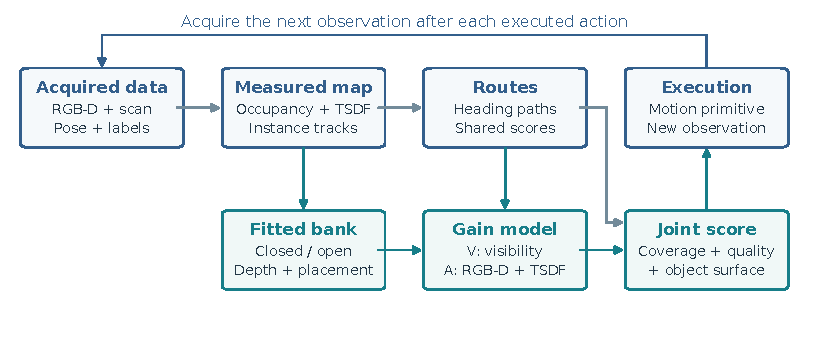
\includegraphics[width=\linewidth]{figures/b11_acquired_loop.pdf}
\caption{The evaluated acquired-state loop. Measured mapping and instance support determine candidate routes and the fitted closed/open bank. G/S controls intervene only on the structural prior at a fixed fitted state. V/A controls replace the template-area forecast while sharing that full bank and all other score terms. The original heading-state executor acquires a new observation after every charged primitive. Predicted TSDFs stay separate from the measured map; source-reference geometry is reserved for evaluation. No trained reachability or loop-closure module is implied by this virtual-study diagram.}
\label{fig:b11-acquired-loop}
\end{figure}

\paragraph{Experimental acquisition-aligned reward.}
Visibility in Eq.~\ref{eq:template-area} does not ensure that an observation will add reconstructed surface. We therefore test an optional forward estimator. For each structural alternative, a separate TSDF replays all acquired RGB-D and then fuses images rendered along the candidate route from the current measured mesh plus that alternative. Let $\widehat M_{oh}(r)$ be this forecast mesh, $M_t$ the measured mesh, and $b_{ohj}$ the original strict-free-space acceptance mask. On a hypothesis-owned surface quadrature,
\begin{equation}
\widehat H_t^m(r)=\sum_{o,h}\pi_{o,T}^m(h)
\sum_j a_{ohj}b_{ohj}
\mathbf 1\{d(p_{ohj},M_t)>\tau\}
\mathbf 1\{d(p_{ohj},\widehat M_{oh}(r))\leq\tau\},
\quad \tau=0.05\,\mathrm m.
\label{eq:acquisition-reward}
\end{equation}
This predicts gross newly reconstructed object area; lost and net area are reported separately. It replaces the old measured-point consumption rule, retains measured-support vetoes against free-space contradictions, and never fuses hypothetical observations into the measured map. The fitted probe uses per-structure conditional-mean geometry and a 0.06\,m surface quadrature, rather than the full particle integral. Unknown unmodeled occluders remain absent. This estimator is tested separately from the complete policies below.

